\chapter{系の設定}

この章では, 本研究で扱う系の設定について説明する. 

2次元の気液共存系で, 質量$m$の粒子が$N$個存在することを考え, 系の上下には壁, 左右には周期境界条件を課す. また, 重力を$y$軸負の向きにかけて, 熱流を$y$軸正の向きに流す. この熱流は, 系の上下の領域にそれぞれ異なる温度を設定したlangevin熱浴を使用することによってかけることとし, NVT-MDシミュレーションを実行する. また, 各熱浴の$y$幅は$8\sigma$となるように設定する. (図\ref{fig:system})


\begin{figure}[H]
  \centering
  \caption{}
  \label{fig:system}
  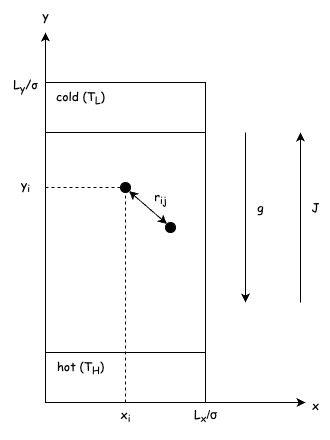
\includegraphics[scale=0.7]{image/system.jpg}
\end{figure}

\section{ハミルトニアン}

\begin{align}
  \label{Hamiltonian}
  H(\Gamma; g)
  &= \sum_{i=1}^{N}
  \left[
    \frac{{\bm{p}_i}^2}{2m} 
    + \sum_{j > i}^{N}
      \tilde{\phi}_{\text{LJ}}^{\text{pair}}(r_{ij})
    + mgy_i
    + V^{\text{wall}} (y_i)
  \right] 
\end{align}

第1項から第4項まで順に, 運動エネルギー, 粒子-粒子間相互作用ポテンシャル, 重力ポテンシャル, 壁-粒子間相互作用ポテンシャルである. 以降, 本節はこのハミルトニアンに至るまでの過程を述べる.

\subsection{粒子-粒子間相互作用ポテンシャル}

シミュレーションを行う際に, 典型的な粒子間相互作用ポテンシャルとして, 12-6 Lennard-Jones Potential を採用する.

\begin{align}
  \phi_{\text{LJ}}^{\text{pair}}(r; \varepsilon, \sigma) = 4\varepsilon \qty[\qty(\frac{\sigma}{r})^{12} - \qty(\frac{\sigma}{r})^{6}] 
\end{align}

シミュレーション上では, カットオフ長 $r_{\text{cut}}^{\text{pair}}=3\sigma$ とポテンシャルのシフトアップを考慮して

\begin{align}
  \tilde{\phi}_{\text{LJ}}^{\text{pair}}(r;r_{\text{cut}}^{\text{pair}}) = \qty{\phi_{\text{LJ}}^{\text{pair}}(r) - \phi_{\text{LJ}}^{\text{pair}}(r_{\text{cut}}^{\text{pair}})}\theta \qty(r_{\text{cut}}^{\text{pair}}-r) \\
\end{align}

のように書き換えたポテンシャルを用いている.

\subsection{周期境界条件と最近接イメージ規約}

周期境界条件を考慮すると, 粒子-粒子間相互ポテンシャルの総計はまず以下のように書ける.\cite{MD}

\begin{align}
  \sum_{n_x \in \mathbb{Z}} \sum_{i=1}^{N} \sum_{\substack{j=1 \\ (j \neq i \ \text{for} \ n_{x} = 0)}}^{N} \frac{1}{2} \phi_{\text{LJ}}^{\text{pair}}(|\bm{r}_i -(\bm{r}_j + L_x \bm{e}_x)|) 
\end{align}

ここで, $n_x = 0$; オリジナルセルの中では, 同じ$i,\ j$ペアのポテンシャルエネルギーを2回足すことになるので, ポテンシャルを$1/2$している. その上で, $j = i$の場合は自分自身との相互作用になるため, これは除外する. $n_x \neq 0$の場合, 粒子$j$はイメージ粒子となるため, $j=i$の場合も含めることになる. このときにもダブルカウントがあるので, ポテンシャルを$1/2$している. 

\begin{figure}[H]
  \centering
  \caption{}
  \label{fig:system_periodic}
  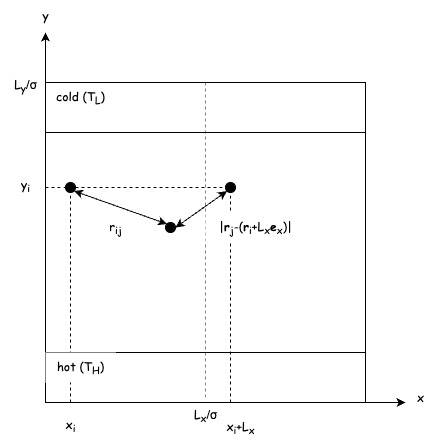
\includegraphics[scale=0.7]{image/system_periodic.jpg}
\end{figure}

注目する系の粒子が常にオリジナルセルの中にとどまっているかのようにMD上で扱うには,

\begin{align}
  x_{i} = x_{i}' \mod L_{x} 
\end{align}

のように,  飛び出した粒子の$x$座標$x_{i}'$を上式のように$x_i$にシフトすれば良い. しかし, 周期境界条件とセットに, 最近接イメージ規約として, 粒子$i$がオリジナル粒子と各イメージ粒子の中で最も近い粒子$j$らとのみ相互作用をすることを課すと, 粒子間の相互ポテンシャルの総計は先ほどよりも簡単に書けるようになる.

\begin{align}
  \sum_{i=1}^{N} \sum_{j > i}^{N} \phi_{\text{LJ}}^{\text{pair}} (r_{ij})
\end{align}

\subsection{壁-粒子間相互作用ポテンシャル}

\begin{align}
  \phi_{\text{LJ}}^{\text{wall}}(r; \varepsilon^{\text{wall}}, \sigma^{\text{wall}}) = 4\varepsilon^{\text{wall}} \qty[\qty(\frac{\sigma^{\text{wall}}}{r})^{12} - \qty(\frac{\sigma^{\text{wall}}}{r})^{6} ] \\
\end{align}

パラメータは以下のようにする.

\begin{align}
  \varepsilon^{\text{wall}} &= \qty(1.0 - \text{R}_\text{d}) \times \varepsilon \\
  \sigma^{\text{wall}} &= \qty(0.5 + \text{R}_\text{t}) \times \sigma \\
  r^{\text{wall}}_{\text{cut}} &= \qty(2^{1/6} + \text{R}_\text{a}) \times \sigma^{\text{wall}}
\end{align}

カットオフ長とシフトアップを考慮して

\begin{align}
  \tilde{\phi}_{\text{LJ}}^{\text{wall}}(r;r_{\text{cut}}^{\text{wall}}) = \qty{\phi_{\text{LJ}}^{\text{wall}}(r) - \phi_{\text{LJ}}^{\text{wall}}(r_{\text{cut}}^{\text{wall}})}\theta \qty(r_{\text{cut}}^{\text{wall}}-r) \\
\end{align}

この系では, $y=0$と$y=L_y$に壁がついている. よって, 壁ポテンシャルは

\begin{align}
  V^{\text{wall}}(y; L_y) &= \tilde{\phi}_{\text{LJ}}^{\text{wall}}(y;r_{\text{cut}}^{\text{wall}}) + \tilde{\phi}_{\text{LJ}}^{\text{wall}}(L_y - y;r_{\text{cut}}^{\text{wall}})
\end{align}

のように書ける. これまでのことより, ハミルトニアンは式\eqref{Hamiltonian}のように書き表せる.

\begin{align}
    H(\Gamma; g)
    &= \sum_{i=1}^{N}
    \left[
      \frac{{\bm{p}_i}^2}{2m} 
      + \sum_{j > i}^{N}
        \tilde{\phi}_{\text{LJ}}^{\text{pair}}(r_{ij})
      + mgy_i +V^{\text{wall}}(y_i)
    \right] \ \tag*{\eqref{Hamiltonian}} 
\end{align}

\section{熱流}

系の両端に温度制御できるランジュバン熱浴を設計することによって, 熱流を実装することにする.

粒子$i$が熱浴に侵入すると, その粒子の運動は以下のランジュバン方程式に従う. 

\begin{align}
  \label{langevin_r}
  \dot{\bm{r}_i} &= \pdv{H}{\bm{p}_i} \\
  \label{langevin_p}
  \dot{\bm{p}_i} &= - \pdv{H}{\bm{r}_i} - \gamma \dot{\bm{r}_i} + \sqrt{2 \gamma k_{\text{B}}T_{\nu}}\bm{\xi}_i (t) 
\end{align}

式\eqref{langevin_p}の第1項は速度に比例する抵抗力, 第2項はランダムな揺動力であり,$\bm{\xi}_{i}(t)$は以下の条件を満たすホワイトノイズである.

\begin{align}
  \bm{\xi}_{i}(t) &= ({\xi_{i}^{x}(t)}, {\xi_{i}^{y}(t)}, {\xi_{i}^{z}(t)}) \\
  \expval{\xi_{i}^{a}(t)} &= 0 \\
  \expval{\xi_{i}^{a}(t)\xi_{j}^{b}(t')} &= \delta_{i,j} \delta_{a,b}\delta (t-t')
\end{align}

粒子がそれぞれの熱浴に侵入していないときには$\gamma=0$となり, 正準方程式に従うようになる. 

\begin{align}
  \gamma(y_i) &= 1. \ T_{\nu}(y_i) = T_{\text{H}}. \ (0 < y_i < 8\sigma) \\
  \gamma(y_i) &= 1. \ T_{\nu}(y_i) = T_{\text{L}}. \ (L_y - 8\sigma < y_i < L_y) \\
  \gamma(y_i) &= 0.  \ (8\sigma < y_i < L_y - 8\sigma)
\end{align}
